\documentclass{beamer}

\usepackage{graphicx}

\title{Ancient Cryptography}
\begin{document}

\begin{frame}
	\titlepage
\end{frame}

\begin{frame}{Caesar Cipher}{Ebiil, Tloia!}
	\begin{block}{Description}
		Each letter in the plaintext is replaced with the letter $n$ above it,
		wrapping around. The value of $n$ is kept secret, as the key.

		\[ E_n(x) = (x+n)\mod 26 \]
	\end{block}

	\begin{block}{History}
		The cipher gets its name from Julius Caesar, who used it in his private
		correspondence, with $n = -3$, so $D \rightarrow A$.
	\end{block}
\end{frame}

\begin{frame}{Caesar Cipher}{Cryptanalysis}
	\begin{figure}
		{\centering English Letter Frequency Distribution}
		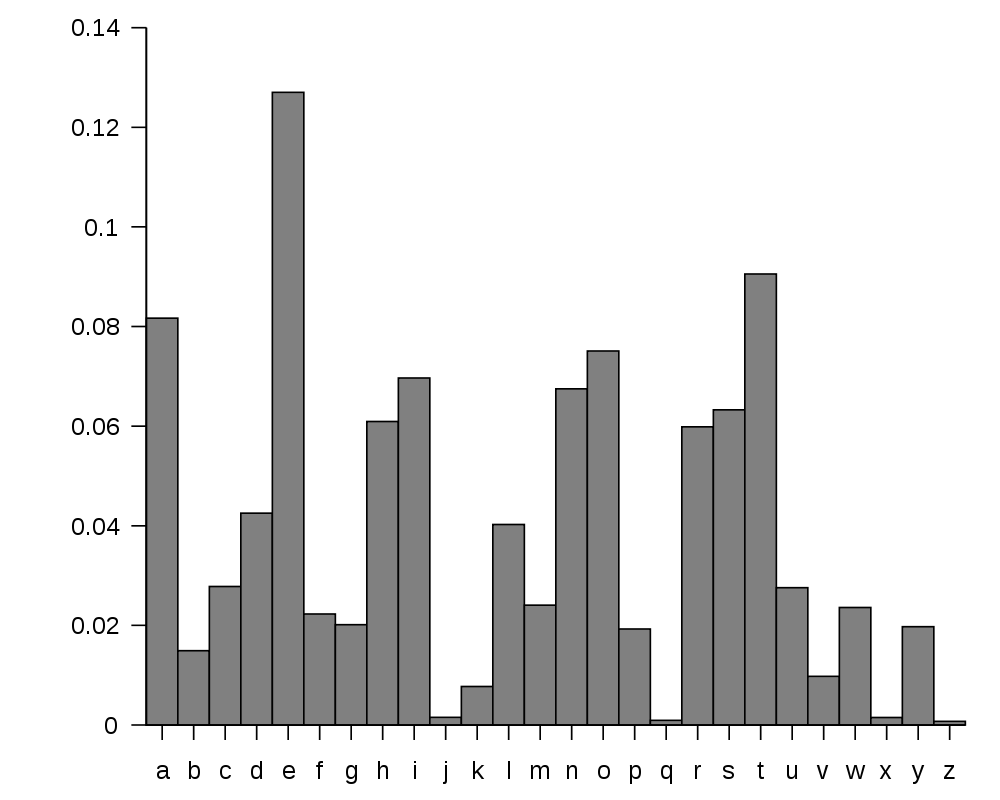
\includegraphics[width=0.9\textwidth]{letter-frequency.png}
	\end{figure}
\end{frame}

\begin{frame}{Vigin\`ere Cipher}
	\begin{block}{Description}
		While a Caesar cipher shifts each letter the same amount, a Viginere
		cipher rotates through a set of shifts according to a keyword. Generally
		$A=0$.
	\end{block}

	For example, if the keyword is {\tt APPLE}, then the first shift will be
	$+A = 0$, the second will be $+P = 15$. The sixth will be the same as the
	first, etc.

	There are no restrictions on the key, but longer is better, and repetitions
	will weaken security.
\end{frame}

% no need for this slide really, but an example would be nice.
\begin{frame}{Vigin\`ere Cipher}
	\begin{block}{History}
		This cipher has been around since roughly 1553 by Giovan Battista
		Bellaso. Blaise de Vigin\`ere actually had nothing to do with its
		invention.
	\end{block}
	\begin{block}{Example}
		We will encrypt {\tt HIDEAWAYPIZZA} using the key {\tt SHENOI}.
	\end{block}
\end{frame}

\begin{frame}{One-Time Pad}
	As the key used in the Vigin\`ere cipher grows longer, it becomes harder to
	analyze and break.

	If the key is the same length as the plaintext {\it (and randomly chosen)},
	it is impossible: Every plaintext is equally likely.

	% ask question: so why don't we just use one-time pads for everything?
\end{frame}

\begin{frame}{Playfair Cipher}
\end{frame}
\end{document}
